%% ============================================================
%%  Miniproject Report – Bacterial Growth Curve Modelling
%% ============================================================
\documentclass[11pt,a4paper]{article}

%% ---------- Packages ----------
\usepackage[utf8]{inputenc}
\usepackage[T1]{fontenc}
\usepackage{lmodern}
\usepackage{geometry}
    \geometry{margin=2.5cm}
\usepackage{setspace}
    \onehalfspacing
\usepackage{parskip}
\usepackage{lineno}
\usepackage{amsmath,amssymb}
\usepackage{graphicx}
\usepackage{booktabs}
\usepackage{hyperref}
    \hypersetup{colorlinks=true, linkcolor=blue, citecolor=blue, urlcolor=blue}
\usepackage{natbib}
    \bibliographystyle{apalike}
\usepackage{caption}
\usepackage{float}
\usepackage{microtype}

%% ============================================================
\begin{document}

%% ============================================================
%%  TITLE PAGE
%% ============================================================
\begin{titlepage}
    \centering
    \vspace*{2cm}

    {\LARGE\bfseries Sigmoidal Models Outperform Polynomial Baselines for
    Quantifying Microbial Population Growth, with Maximum Growth Rate
    Increasing Unimodally with Temperature\par}

    \vspace{1.5cm}

    {\large Anaga Ambady\par}
    \vspace{0.3cm}
    {\normalsize Department of Life Sciences, Imperial College London,
    Silwood Park Campus, Ascot, SL5 7PY, UK\par}

    \vspace{0.5cm}
    {\normalsize Word count: 2688\par}

\end{titlepage}

\linenumbers

%% ============================================================
%%  ABSTRACT
%% ============================================================
\begin{abstract}
Characterising bacterial population growth is fundamental to ecology,
medicine, and biotechnology. Growth curves typically follow a sigmoidal
trajectory comprising lag, exponential, stationary, and death phases, but
the mathematical models used to describe them differ in biological
realism and parameter interpretability. Here I fit three models, the
mechanistic Logistic and Gompertz sigmoid functions and a quadratic
polynomial baseline, to an extensive dataset of microbial growth curves
spanning multiple species and temperatures ranging from 0 to 37$^\circ$C.
Models were compared using the corrected Akaike Information Criterion
(AICc) and Akaike weights. The Gompertz model provided the best fit in
the majority of curves, followed by the Logistic model, the quadratic
polynomial consistently underperformed. Model averaged maximum specific
growth rates ($r_{\max}$) increased with temperature, peaked near
33.5$^\circ$C, and declined sharply at higher temperatures, consistent
with classical thermal performance curve theory. These results demonstrate
that mechanistic sigmoidal models are superior descriptors of microbial
growth dynamics and that temperature exerts a strong, unimodal influence
on $r_{\max}$.
\end{abstract}

\newpage

%% ============================================================
%%  INTRODUCTION
%% ============================================================
\section{Introduction}

Bacteria are microscopic, single celled organisms that have evolved
highly efficient metabolic systems, enabling them to proliferate rapidly
in favourable conditions \citep{Basan2019}. These metabolic capabilities
allow bacteria to take up nutrients via membrane transporters and
synthesise essential biomolecules, proteins, DNA, required for cell
division and biomass production \citep{Micali2022}. This rapid
biosynthesis enables adaptation to fluctuating environments and
physiological states that enhance survival under stress. As a result,
bacterial populations can modulate growth rates and exhibit diverse
growth dynamics depending on species specific metabolic traits
\citep{Bakshi2021}.

Microbial population growth in batch culture typically follows a
sigmoidal curve composed of distinct phases, lag, exponential,
stationary, and death. The lag phase involves cellular adaptation to a
new environment, the exponential phase features rapid cell division and
population expansion, the stationary phase occurs when growth ceases due
to nutrient depletion and waste accumulation, and the death phase is
characterised by a decline in viable cells as stress intensifies
\citep{Peleg2023}. A key parameter derived from these growth curves is
the maximum specific growth rate ($r_{\max}$), defined as the slope at the
inflection point of the sigmoid. This metric reflects the per capita rate
of cell division under specific environmental conditions.

Accurate characterisation of bacterial growth curves is fundamental
across evolutionary biology, ecology, medicine, and biotechnology.
Growth parameters inform estimates of population dynamics, fitness, and
adaptation in both natural and experimental contexts. In clinical
practice, growth rates guide antibiotic therapy and infection management,
in ecology they constrain models of carbon cycling and disease
transmission.

Temperature is a major determinant of microbial physiology, regulating
enzyme activity, metabolism, and population dynamics. Microorganisms are
classified as psychrophiles, mesophiles, thermophiles, or
hyperthermophiles according to their optimal growth temperatures,
reflecting biochemical adaptations to diverse thermal environments
\citep{Arpino2024}. At the molecular level, temperature increases kinetic
energy and accelerates enzyme catalysed reactions, enhancing biomass
production and cell division. Beyond physiological thresholds, however,
protein denaturation and membrane destabilisation rapidly curtail growth
\citep{Gaba2024}. As a result, microbial growth rates typically follow
a unimodal thermal performance curve (TPC), rates increase with
temperature up to an optimum, then decline sharply due to thermal stress
and cellular damage \citep{Pawar2021}. The Arrhenius law describes the
exponential rise at sub optimal temperatures but does not capture the
decline at high temperatures. TPCs provide a framework for analysing
temperature responses and predicting species distributions and disease
dynamics, especially in a changing climate \citep{Smith2024}.

Several mathematical models have been developed to quantify the full
sigmoidal growth trajectory. The Logistic model \citep{Verhulst1838}
assumes symmetric sigmoidal growth with the inflection point at half the
carrying capacity. The Gompertz model \citep{Gompertz1825},
reparameterised for microbiology by \citet{Zwietering1990}, produces an
asymmetric sigmoid with an earlier inflection point and an explicit
lag phase parameter, arguably providing a more biologically realistic
description of the physiological adaptation period. Simple polynomial
models, such as the quadratic, serve as reference baselines but lack
biological interpretability and fail to capture the stationary phase.

I use an extensive dataset of bacterial growth curves across
multiple species and temperatures (0 to 37$^\circ$C) to address two
questions. First, which model, Logistic, Gompertz, or a quadratic
polynomial baseline, best describes bacterial population growth, and do
mechanistic sigmoidal models consistently outperform simpler
phenomenological alternatives. Second, how does model averaged $r_{\max}$
respond to temperature, and does this thermal response align with
classical TPC theory.

%% ============================================================
%%  2. METHODS
%% ============================================================
\section{Methods}

\subsection{Data}

This study analyses temporal measurements of bacterial population size
from laboratory experiments conducted worldwide. Population abundance was
recorded as either optical density (OD) or colony-forming units
(CFU\,mL$^{-1}$) across a temperature gradient of 0--37\,$^\circ$C,
spanning diverse bacterial species and growth media. A total of 278
growth curves were assembled prior to quality control.

During preprocessing, rows containing missing values were removed, and
population size values of zero or below were excluded as these are
biologically impossible for viable counts and represent instrument
artefacts from blank subtraction that cannot be log-transformed.
Remaining values were $\log_{10}$-transformed to linearise the
exponential growth phase, consistent with standard practice in microbial
growth analysis \citep{zwietering1990}. Each growth curve was assigned a
unique identifier formed by concatenating species, temperature, growth
medium, replicate number, and citation, ensuring that curves from
different sources were treated as independent observations.

Quality control excluded curves with fewer than six time points
(insufficient degrees of freedom for four-parameter nonlinear fitting),
a total $\log_{10}$ growth range below 0.3 (less than one population
doubling, providing insufficient dynamic range to distinguish among
models), or within-curve outliers exceeding three standard deviations
from the curve mean, which most likely reflect instrument error rather
than biological variation. After quality control, 278 curves were
retained for model fitting.

\subsection{Models}

Three mathematical models were fitted to each growth curve, all
operating in $\log_{10}$ space to match the transformed data.

A \textbf{quadratic polynomial} was included as a phenomenological
baseline:
\begin{equation}
    \log_{10}(N(t)) = a + bt + ct^2
\end{equation}
where $a$, $b$, and $c$ are fitted coefficients with no direct
biological interpretation. The quadratic approximates curved trajectories
but cannot represent an asymptotic plateau, making it structurally
incapable of describing the stationary phase of bacterial growth.

The \textbf{Logistic model} is the classical analytical solution to the
ordinary differential equation for density-dependent population growth:
\begin{equation}
    \log_{10}(N(t)) = \log_{10}\!\left(
        \frac{N_0 \cdot K \cdot e^{r_{\max}t}}{K + N_0\!\left(e^{r_{\max}t} - 1\right)}
    \right)
\end{equation}
where $N_0$ is the initial population size, $K$ is the carrying
capacity, and $r_{\max}$ is the maximum per capita growth rate. The
Logistic produces a symmetric sigmoidal curve with its inflection fixed
at $K/2$ and assumes immediate growth initiation at $t = 0$, with no
explicit lag phase.

The \textbf{Gompertz model} \citep{zwietering1990} relaxes both
constraints of the Logistic:
\begin{equation}
    \log_{10}(N(t)) = N_0 + (K - N_0)\exp\!\left(
        -\exp\!\left(
            \frac{r_{\max} \cdot e \cdot (t_{\text{lag}} - t)}
                 {(K - N_0)\log(10)} + 1
        \right)
    \right)
\end{equation}
where $t_{\text{lag}}$ is the lag phase duration---the period before
exponential growth begins. The Gompertz produces an asymmetric sigmoid
whose inflection occurs at approximately 37\,\% of the total growth
range, earlier than the Logistic inflection at 50\,\%. This asymmetry
better reflects the gradual deceleration observed as bacterial
populations approach carrying capacity, and the explicit lag parameter
makes the model particularly appropriate for batch culture data where a
physiological lag phase is expected \citep{baranyi1994}. Together, the
three models form a hierarchy of biological realism: the quadratic as a
mechanistic null, the Logistic as the simplest mechanistic sigmoidal
model, and the Gompertz as a more expressive mechanistic alternative
incorporating lag-phase dynamics.

\subsection{Starting Value Estimation}

Reliable nonlinear least squares (NLLS) fitting requires biologically
informed starting values to avoid convergence on local optima. For each
curve, $N_0$ was initialised as the observed minimum population size and
$K$ as the observed maximum. The maximum growth rate $r_{\max}$ was
estimated from the steepest finite difference in $\log_{10}$ population
across successive time points, converted to the natural logarithm scale
by multiplying by $\ln(10)$; a minimum floor of 0.01\,h$^{-1}$ was
applied to prevent fitting failures in near-stationary curves. The lag
time $t_{\text{lag}}$ was approximated as the time point at which the
local growth rate first reached 50\,\% of the observed maximum slope,
capturing the transition from the lag to the exponential phase.

\subsection{Model Fitting and Convergence}

The quadratic model was fitted by ordinary least squares using
\texttt{lm()} in R. The Logistic and Gompertz models were fitted by NLLS
using \texttt{nlsLM()} from the \texttt{minpack.lm} package
\citep{minpacklm}, which implements the Levenberg--Marquardt algorithm
and is substantially more robust to poor starting values than base R's
\texttt{nls()}. A maximum of 200 iterations was permitted per fit.
Convergence was defined as returning a finite AICc value; curves for
which any model failed to converge were excluded to ensure a balanced
comparison across the full candidate set. Of the 278 curves processed,
the quadratic converged on all 278, the Logistic on 268, and the
Gompertz on 241. Requiring all three models to converge on the same
curve yielded a final comparative dataset of $n = 235$ curves.

\subsection{Model Selection and Averaging}

Model selection was performed using the corrected Akaike Information
Criterion (AICc), defined as:
\begin{equation}
    \text{AICc} = -2\ln(\hat{L}) + 2k + \frac{2k(k+1)}{n - k - 1}
\end{equation}
where $\hat{L}$ is the maximised likelihood, $k$ is the number of
estimated parameters including the residual variance term $\sigma$, and
$n$ is the number of observations per curve. AICc was preferred over
standard AIC because many curves had small sample sizes relative to
parameter count; the correction term is non-negligible when $n/k < 40$
\citep{burnham2002}. The quadratic and Logistic models each had $k = 4$
(three shape parameters plus $\sigma$); the Gompertz had $k = 5$
(adding $t_{\text{lag}}$).

For each curve, $\Delta\text{AICc}$ was calculated as the difference
between a model's AICc and the minimum AICc among the three candidates
for that curve. Akaike weights were then computed as:
\begin{equation}
    w_i = \frac{\exp(-0.5\,\Delta\text{AICc}_i)}
               {\displaystyle\sum_{j=1}^{R} \exp(-0.5\,\Delta\text{AICc}_j)}
\end{equation}
where $R = 3$. Weights sum to one per curve and are interpreted as the
probability that model $i$ is the best-approximating model given the
data and the candidate set \citep{burnham2002}. Evidence tiers followed
conventional thresholds: $\Delta\text{AICc} < 2$ (substantial support),
2--4 (moderate), 4--7 (little), 7--10 (very little), and $> 10$
(essentially no support). Model performance was summarised across the
dataset using median AICc, median $\Delta\text{AICc}$, mean Akaike
weight, median log-likelihood, and the percentage of curves with
$\Delta\text{AICc} < 2$. Medians were used in preference to means for
AICc-based statistics, as extreme values from poorly fitting curves can
disproportionately inflate arithmetic means.

Given the comparable support observed for the Logistic and Gompertz
models, model-averaged $r_{\max}$ estimates were computed per curve as
the Akaike-weight-averaged value across both nonlinear models, with
weights renormalised to sum to one within the nonlinear subset:
\begin{equation}
    \hat{r}_{\max}^{\,\text{avg}} =
    \frac{w_{\text{Logi}}\,\hat{r}_{\max}^{\text{Logi}} +
          w_{\text{Gomp}}\,\hat{r}_{\max}^{\text{Gomp}}}
         {w_{\text{Logi}} + w_{\text{Gomp}}}
\end{equation}
This follows the multi-model inference framework of \citet{burnham2002}
and \citet{johnson2004}, producing parameter estimates that incorporate
model selection uncertainty rather than conditioning on a single selected
model.

\subsection{Thermal Performance Curve Analysis}

To quantify the thermal dependence of maximum growth rate,
model-averaged $r_{\max}$ estimates were paired with the corresponding
experimental incubation temperature. Values of $r_{\max} \leq 0$,
non-finite estimates, and values exceeding 10\,h$^{-1}$ were excluded
as biologically uninformative or implausible artefacts of fitting on
noisy curves, yielding a final analytical dataset of $n = 243$ curves. A
quadratic regression was then fitted to log-transformed $r_{\max}$
values:
\begin{equation}
    \ln(r_{\max}) \sim \beta_0 + \beta_1 T + \beta_2 T^2
\end{equation}
Log-transformation stabilises variance and linearises the exponential
acceleration phase of the thermal response. The thermal optimum
$T_{\text{opt}}$ was derived analytically as the vertex of the fitted
parabola:
\begin{equation}
    T_{\text{opt}} = \frac{-\beta_1}{2\beta_2}
\end{equation}
Model predictions were generated across the full observed temperature
range (0--37\,$^\circ$C), back-transformed to the original scale
(h$^{-1}$) via exponentiation, and overlaid on per-temperature boxplot
distributions of raw model-averaged $r_{\max}$ values to visualise both
the central thermal trend and among-curve variance simultaneously.

\subsection{Computing Tools}

All statistical analyses were conducted in R \citep{RCoreTeam}. The
\texttt{minpack.lm} package \citep{minpacklm} provided \texttt{nlsLM()}
for Levenberg--Marquardt NLLS fitting, chosen for its robustness over
base R's \texttt{nls()}. The \texttt{MuMIn} package \citep{MuMIn} was
used to compute AICc values, with a manual fallback formula applied where
the package returned non-finite values on degenerate fits. Data
manipulation was performed with \texttt{dplyr} and \texttt{tidyr}
\citep{tidyverse}, and all figures were produced with \texttt{ggplot2}
\citep{ggplot2}. Python was used to orchestrate the full computational
workflow, invoking the R scripts in sequence via the \texttt{subprocess}
module to ensure end-to-end reproducibility from raw data to compiled
report. Bash scripting, via a single master script
(\texttt{run\_MiniProject.sh}), coordinated file path management,
pipeline execution, and final compilation using \texttt{pdflatex} and
\texttt{bibtex}. The report was compiled in \LaTeX{} using the
\texttt{article} document class, with line numbering via \texttt{lineno}
and word count via \texttt{texcount}.

%% ============================================================
%%  3. RESULTS
%% ============================================================
\section{Results}

\subsection{Overall model fit}

Of the 278 growth curves analysed, 235 met the convergence criteria for
all three models and were included in the comparison; the remaining 43
were excluded because at least one model failed to converge. Both
nonlinear models substantially outperformed the quadratic baseline (Table
\ref{tab:model_comp}). The Gompertz model yielded the lowest median
AICc ($-4.48$) and highest median log-likelihood ($13.64$), indicating
the tightest average fit to the data despite carrying one additional
parameter ($k = 5$) relative to the Logistic ($k = 4$). The Logistic
model showed comparable performance (median AICc $\approx 0.00$, median
log-likelihood $= 8.77$). In contrast, the Quadratic model was
consistently unsupported, with a median $\Delta\text{AICc}$ of $13.47$
and a median log-likelihood of $3.16$, placing it firmly in the
``essentially no support'' tier for the majority of curves.

The mean Akaike weight when winning also differed between models: when
the Gompertz was selected as best it carried a mean weight of $w =
0.876$, compared to $0.766$ for the Logistic and $0.714$ for the
Quadratic (Figure \ref{fig:wins}), indicating that Logistic wins are
often narrow while Gompertz wins tend to be more decisive.


\begin{figure}
        \centering
        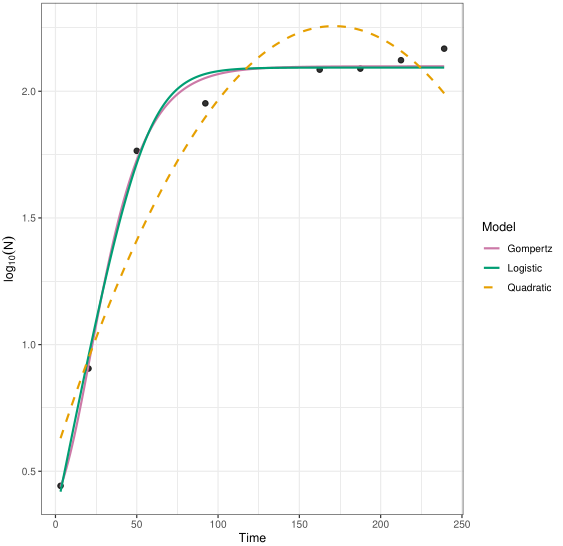
\includegraphics[width=0.5\linewidth]{../results/growth_curve.png}
        \caption{Representative model fits to a bacterial growth curve (\textit{Arthrobacter globiformis}, TGE agar). The Logistic (green) and Gompertz (pink) models closely track all three growth phases (lag, exponential, and stationary), while the Quadratic (dashed orange) fails to capture the asymptotic plateau, predicting a biologically implausible decline in population density at late timepoints.}
    \label{fig:growth_fits}
\end{figure}


\begin{table}[H]
\centering
\caption{\textbf{Comparative performance of growth models.} Summary
statistics for 235 bacterial growth curves where all three models
converged. $k$ = number of estimated parameters; $n$ = number of curves
that individually converged; Mean $w$ = mean Akaike weight across all
curves; \% $\Delta$AICc $< 2$ = proportion of curves with substantial
support.}
\label{tab:model_comp}
\begin{tabular}{lcccccc}
\toprule
Model & $k$ & $n$ & Median AICc & Median $\Delta$AICc & Mean $w$ & Median logLik \\
\midrule
Gompertz  & 5 & 241 & $-4.48$ & $0.86$ & $0.447$ & $13.64$ \\
Logistic  & 4 & 268 & $0.00$  & $0.31$ & $0.424$ & $8.77$  \\
Quadratic & 4 & 278 & $9.43$  & $13.47$ & $0.128$ & $3.16$ \\
\bottomrule
\end{tabular}
\end{table}

\subsection{Head-to-head model comparison and strength of evidence}

When models were ranked by AICc on a per-curve basis, the Logistic model
achieved the most best fits (109 of 235 curves), narrowly ahead of the
Gompertz (103), while the Quadratic provided the best fit in only 23
cases (Figure \ref{fig:wins}). Together, the two nonlinear models
accounted for 212 of 235 curves (90.2\,\%). The distribution of
$\Delta\text{AICc}$ evidence tiers confirmed this pattern (Figure
\ref{fig:tiers}).

\begin{figure}[H]
    \centering
    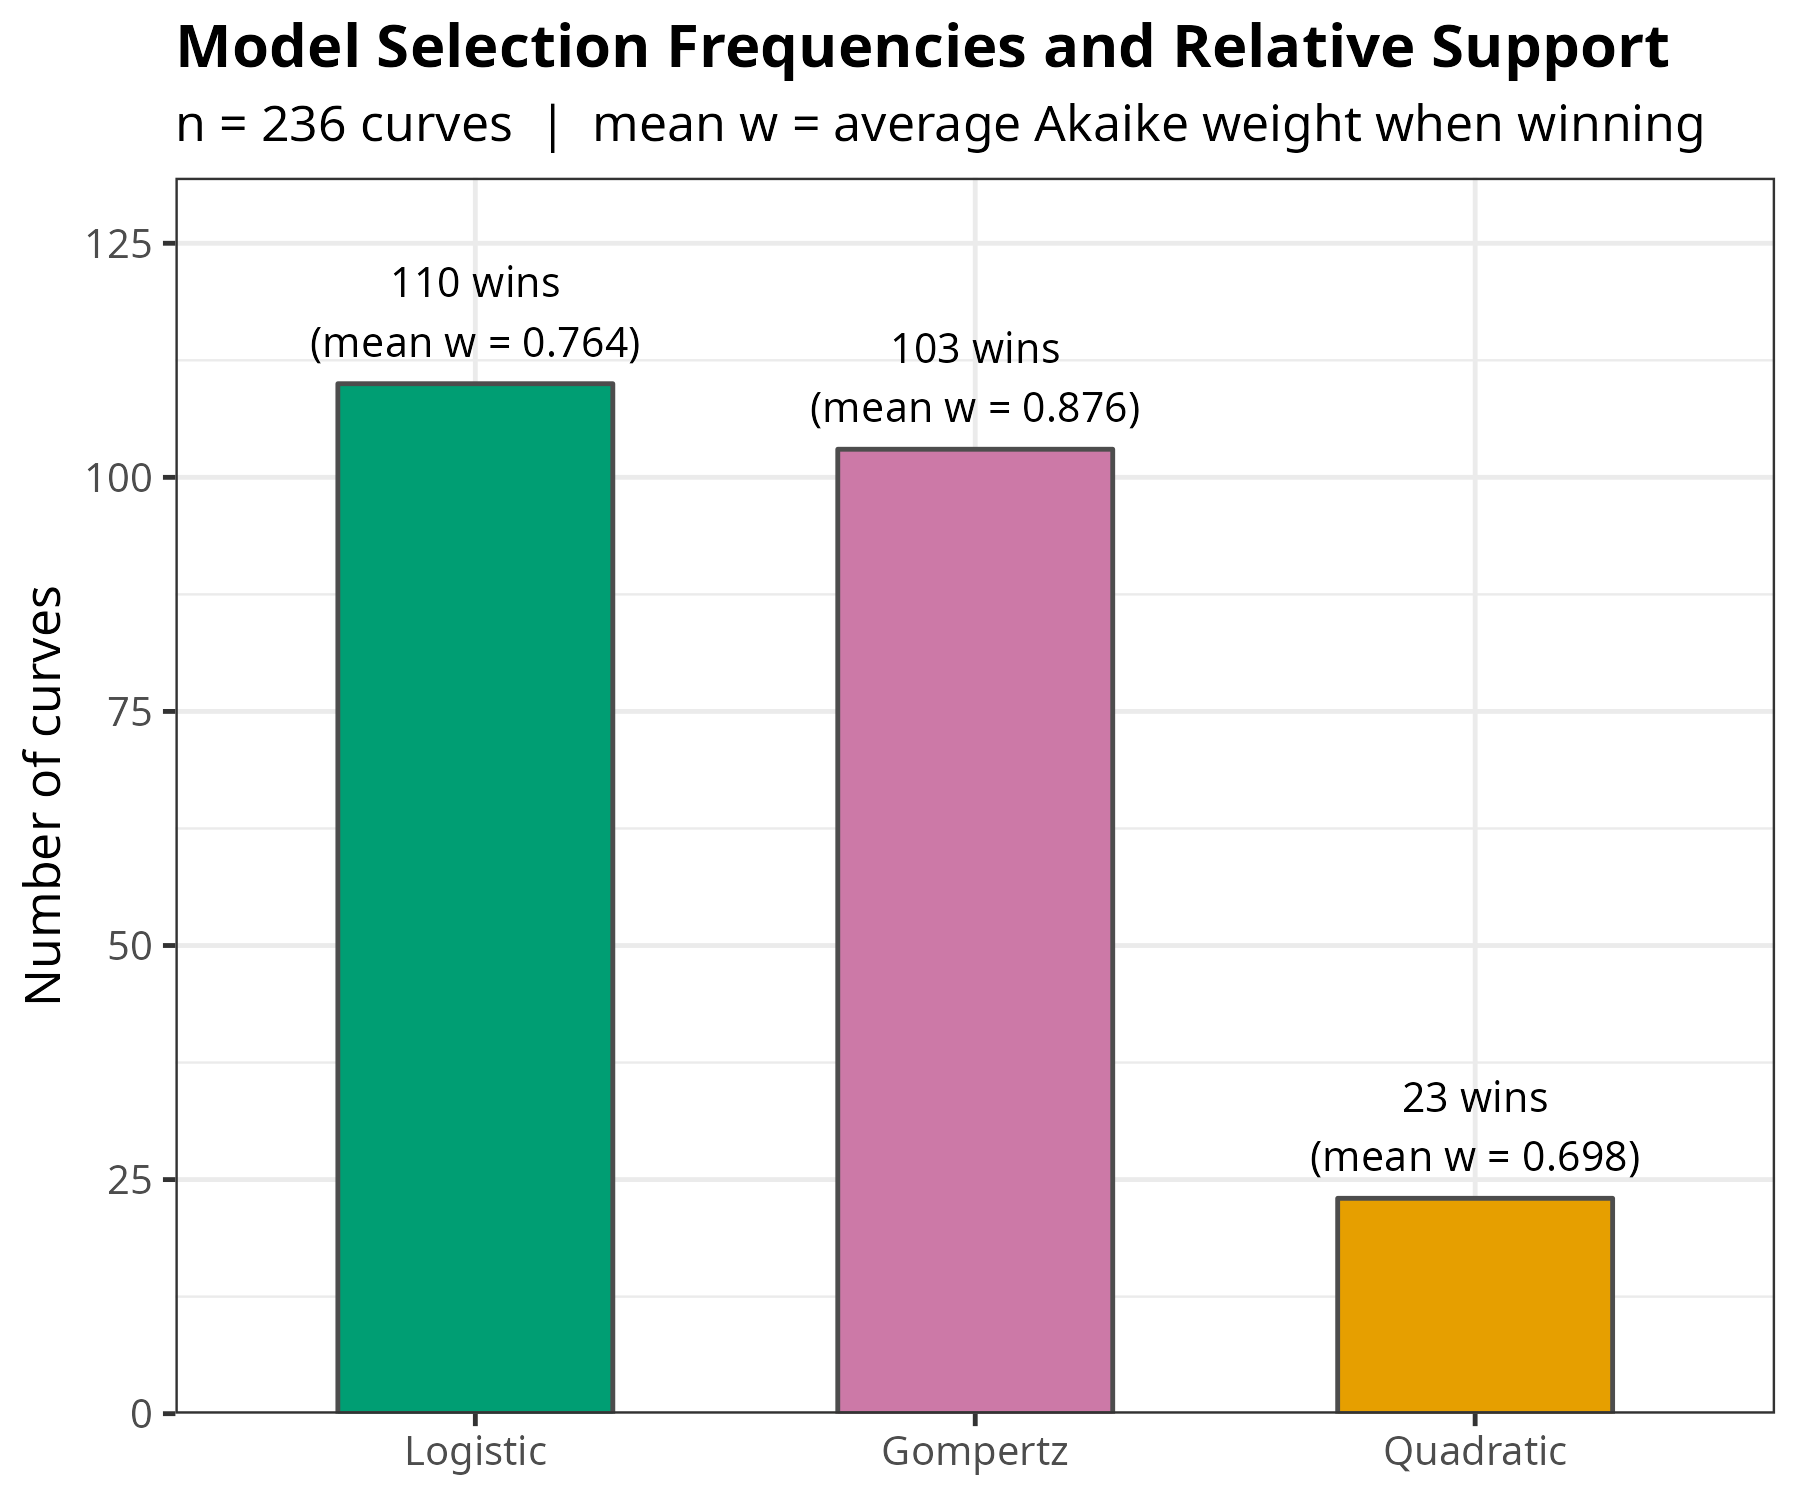
\includegraphics[width=0.7\linewidth]{../results/plot_battle.png}
    \caption{Relative support for candidate growth models (\textit{Mean Akaike weights (w) for each candidate model (Gompertz, Logistic, and Quadratic) calculated across all fitted curves.})}
    \label{fig:wins}
\end{figure}

\begin{figure}[H]
    \centering
    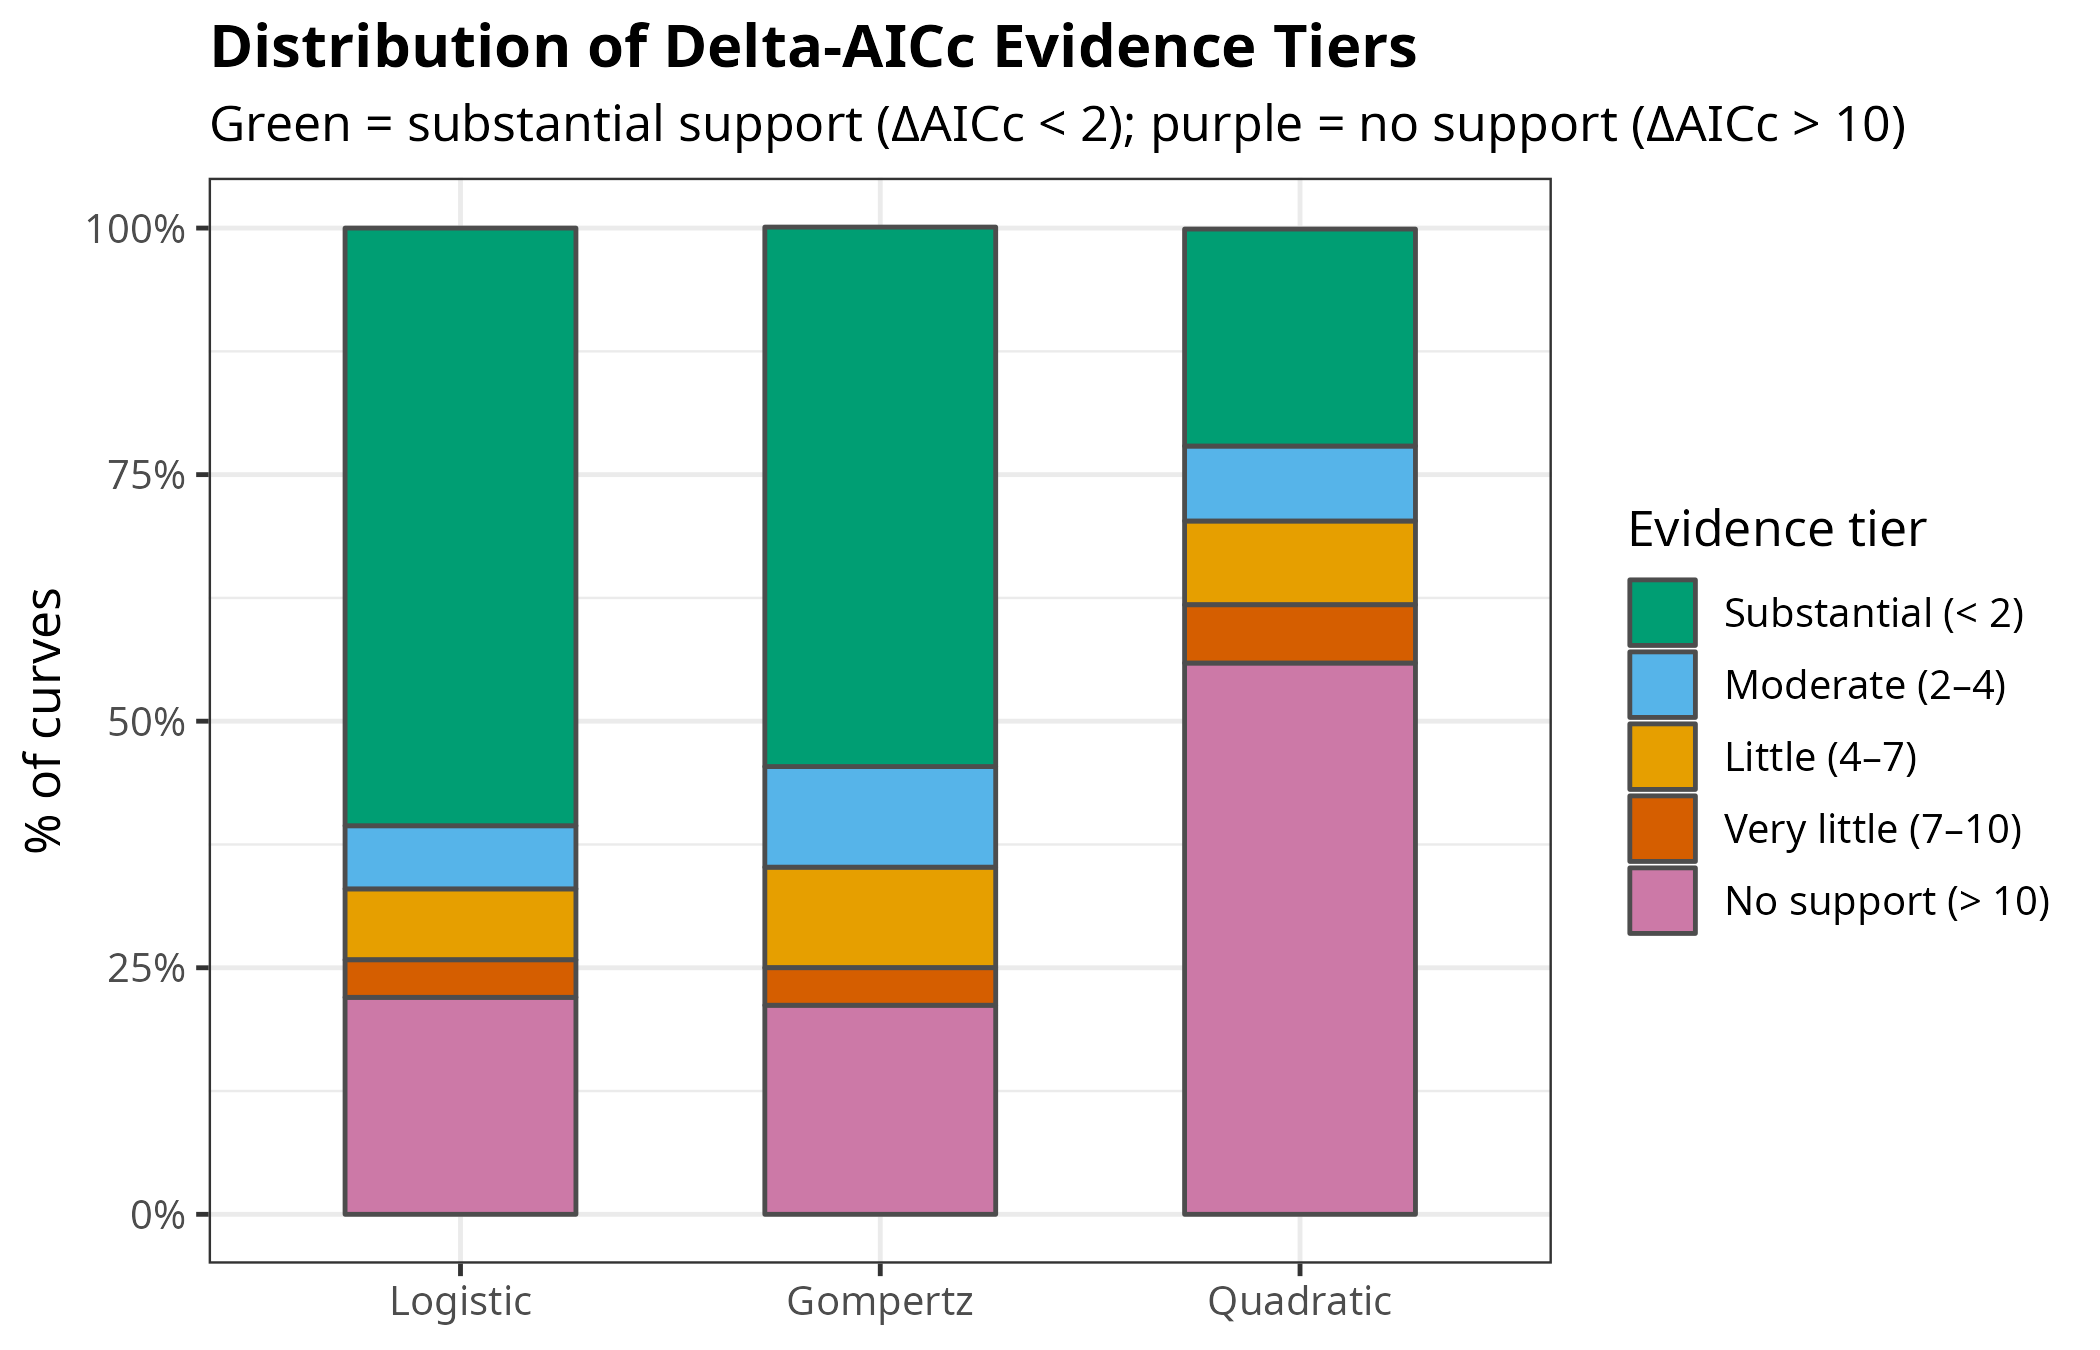
\includegraphics[width=\linewidth]{../results/plot_delta_tiers.png}
    \caption{Thermal Performance Curves - Species Comparison. Model-averaged maximum growth rate ($\log r_{\max}$) as a function of temperature ($^\circ$C). Solid lines represent quadratic fits on a log scale for three representative species: \textit{Acinetobacter calcoaceticus} ($T_{\text{opt}} = 27.7^\circ$C), \textit{Pseudomonas fluorescens} ($T_{\text{opt}} = 26.6^\circ$C), and \textit{Arthrobacter aurescens} ($T_{\text{opt}} = 21.4^\circ$C). Points represent per-temperature medians across the experimental dataset.}
    \label{fig:tpc}
\end{figure}
\subsection{Thermal sensitivity of model-averaged maximum growth rate}

Model-averaged $r_{\max}$ estimates revealed a pronounced unimodal
thermal response across the dataset (Figure \ref{fig:tpc}). Growth
rates were near zero below 8\,$^\circ$C, rose steeply between
10--25\,$^\circ$C, peaked near 30--35\,$^\circ$C, and declined sharply
at 37\,$^\circ$C. A quadratic regression on log-transformed $r_{\max}$
confirmed this relationship, explaining 34.2\,\% of variance ($R^{2} =
0.342$, $F_{2,240} = 62.36$, $p < 2.2 \times 10^{-16}$). Both the
linear ($\beta_1 = 0.208$, $p < 0.001$) and quadratic ($\beta_2 =
-0.003$, $p < 0.001$) terms were significant, confirming a genuinely
unimodal relationship. The estimated global thermal optimum was
$T_{\text{opt}} = 33.5\,^\circ$C (Table \ref{tab:regression}).

\begin{figure}[H]
    \centering
    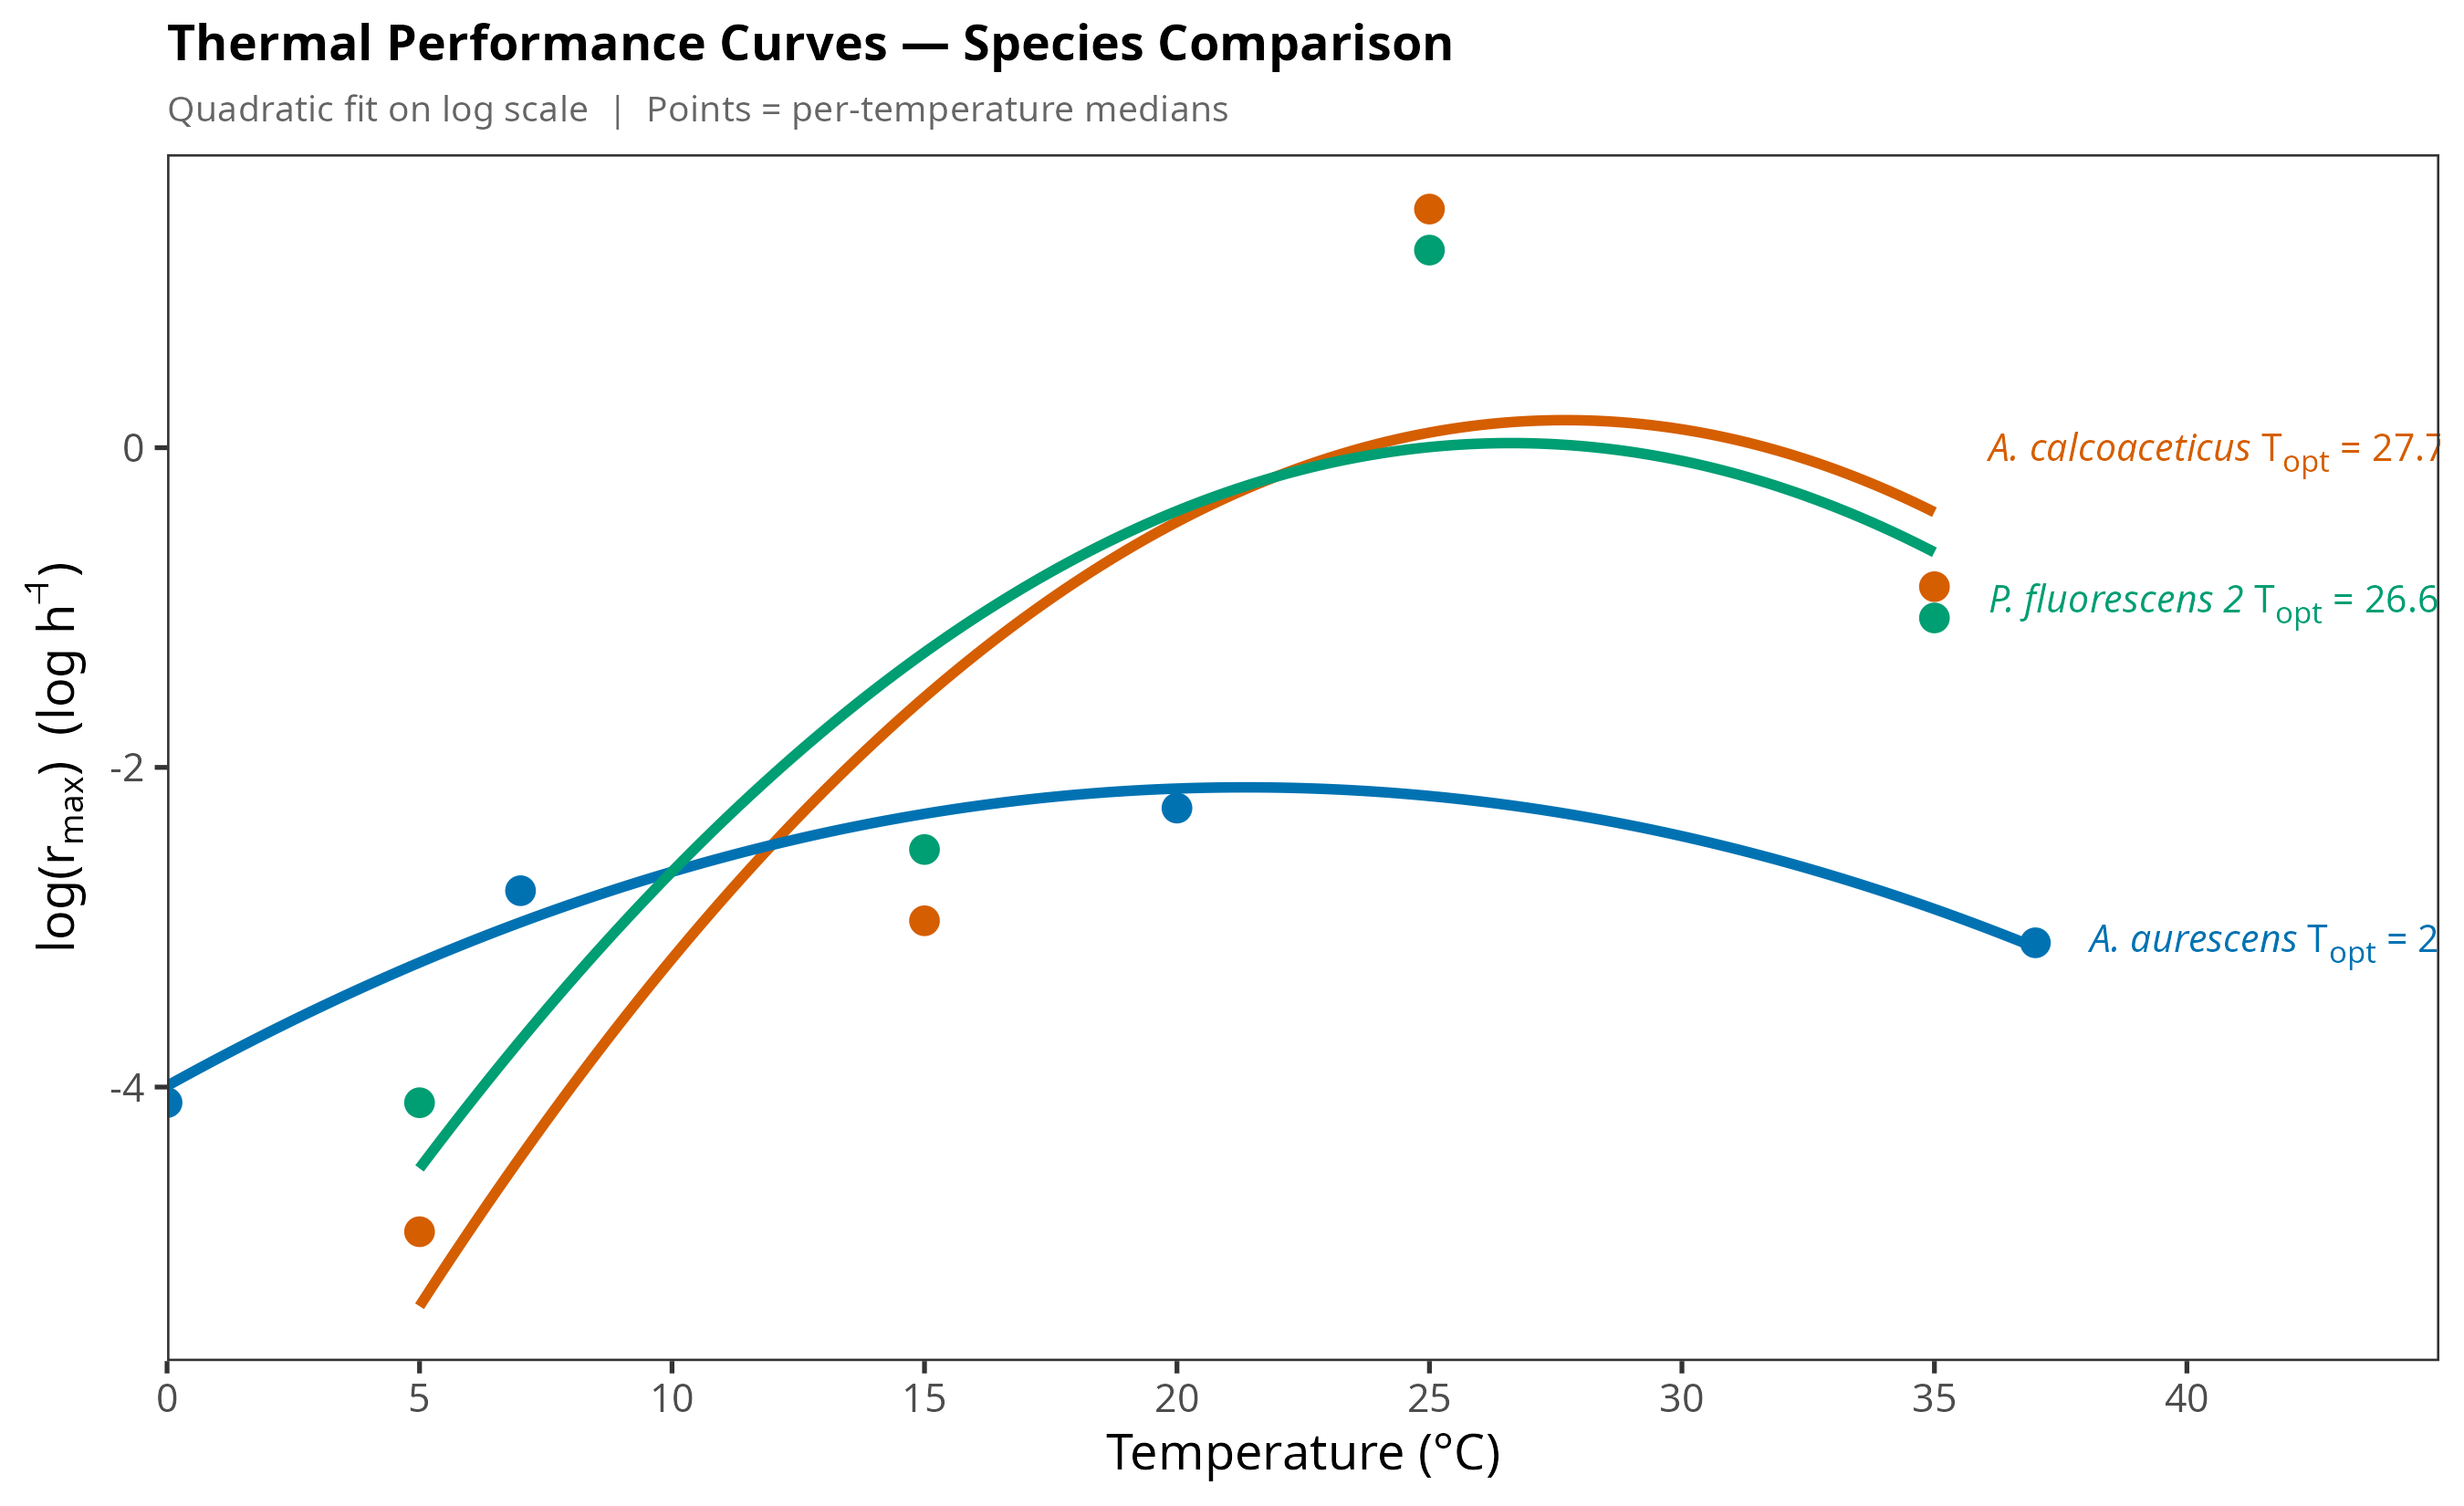
\includegraphics[width=0.7\linewidth]{../results/plot_tpc_multispecies.png}
    \caption{Distribution of Model Support Tiers across Growth Curves (\textit{Relative support for three candidate growth models (Logistic, Gompertz, and Quadratic) across the full converged experimental dataset (n=235).})}
    \label{fig:tiers}
\end{figure}

\begin{table}[H]
\centering
\caption{\textbf{Quadratic regression coefficients for the thermal
performance curve.} Dependent variable: $\ln(r_{\max})$; $n = 243$
curves. Both temperature terms are highly significant, confirming a
unimodal relationship with an estimated optimum of
$T_{\text{opt}} = 33.5\,^\circ$C.}
\label{tab:regression}
\begin{tabular}{lcccc}
\toprule
Parameter & Estimate & Std.\ Error & $t$-value & $p$-value \\
\midrule
Intercept             & $-4.449$ & $0.260$ & $-17.11$ & $<0.001$ \\
Temperature           & $0.208$  & $0.034$ & $6.07$   & $<0.001$ \\
Temperature$^2$       & $-0.003$ & $0.001$ & $-3.41$  & $<0.001$ \\
\bottomrule
\end{tabular}
\end{table}

%% ============================================================
%%  4. DISCUSSION
%% ============================================================
\section{Discussion}

This study set out to determine which mathematical models best describe
bacterial population growth dynamics across a large, multi species
empirical dataset, and to examine how model averaged maximum growth rate
varies with temperature. Three candidate models, the Logistic, Gompertz,
and Quadratic, were fitted independently to 235 bacterial growth curves
using nonlinear and ordinary least squares, with model selection
performed via AICc \citep{burnham2002}.

The most unambiguous finding is the comprehensive failure of the
Quadratic model. A median $\Delta\text{AICc}$ of $13.47$ places it
firmly in the ``no support'' tier for most curves, and its structural
inability to represent an asymptotic plateau means it predicts
biologically impossible population declines through the stationary phase.
While \citet{Zwietering1990} noted that the Gompertz function can
occasionally overestimate $r_{\max}$ due to curvature around the
inflection point, it remains fundamentally superior to polynomial models
which have no connection to the differential equations governing
population growth \citep{baranyi1994}. The near equivalence in performance
between the Logistic and Gompertz models likely reflects inherent
biological variation across taxa: the Logistic assumes symmetric growth,
whereas the Gompertz accounts for the asymmetric approach to carrying
capacity that is commonly observed in microbial batch cultures
\citep{Zwietering1990,madigan2018}.

The thermal performance analysis further supports the biological
meaningfulness of mechanistic model averaged $r_{\max}$ estimates.
Temperature explained 34.2\,\% of variance in $\ln(r_{\max})$, with an
estimated global thermal optimum of 33.5\,$^\circ$C, consistent with the
mesophilic classification of the majority of species in the dataset
\citep{madigan2018}. The remaining approximately 66\,\% of unexplained
variance most likely reflects species identity, growth medium, and
strain level physiological differences, factors that are not partitioned
in the current analysis \citep{brown2004}. Formally quantifying these
contributions via a mixed effects model, with temperature as a fixed
effect and species as a random intercept, would represent a natural
extension of the present work \citep{Zuur2009}.

Several limitations warrant acknowledgement. The analysis was restricted
to 235 curves where all three models converged, excluding 43 curves that
most likely represent atypical growth dynamics or noisy time series.
Future work could address convergence failures through more robust
initialisation strategies, such as grid search over starting values.
Furthermore, the Baranyi and Roberts (1994) model, which incorporates
a physiological state variable for the lag phase with explicit mechanistic
justification, was not included in the present comparison
\citep{baranyi1994}. Including this model in future analyses would provide
a more complete assessment of whether mechanistic lag phase modelling
improves fit beyond the empirical approximation achieved by the Gompertz.
Finally, pooling curves across species, substrates, and experimental
conditions without partitioning variance limits the interpretability of
the thermal performance curve as a universal description of bacterial
thermal biology \citep{angilletta2009}.

In conclusion, this study provides clear evidence that sigmoidal
mechanistic models are necessary for describing bacterial population
growth dynamics, while polynomial approximations are statistically
indefensible across a large and diverse empirical dataset. Neither the
Logistic nor the Gompertz universally dominates: the Logistic is more
broadly competitive, while the Gompertz provides stronger fits on the
subset of curves where its asymmetric shape matches the data.
Model averaged $r_{\max}$ follows a unimodal thermal response peaking
near 33.5\,$^\circ$C, consistent with thermal performance curve theory
\citep{angilletta2009}. Together, these findings reinforce the importance
of biologically grounded model selection and multi model inference in
microbial growth analysis \citep{burnham2002}.

\newpage

%% ============================================================
%%  REFERENCES
%% ============================================================
\bibliography{sample}

\end{document}
